\chapter{Affine Spaces and Vectors: A Geometric Foundation}

\section{Introduction: From High School Geometry to University Mathematics}

In high school geometry, we often think of vectors as ``arrows'' that have a length and a direction. We learn that two arrows are ``equivalent'' (or represent the same vector) if they have the same length and direction, even if they start at different locations.

In this chapter, we formalize this intuition using the language of $\mathbb{R}^n$. We will see that vectors can be thought of as ``translations'' or ``shifts'' of the space, and that many geometric properties we are familiar with (like congruence) are simply properties that remain unchanged when we shift figures around.

This geometric foundation will prove essential in Chapter 3 when we introduce the O notation for comparing functions via norms, and in Chapter 4 when we define derivatives as linear approximations.

\section{Points and Translations in $\mathbb{R}^n$}

\subsection{The Space $\mathbb{R}^n$}
We define the space $\mathbb{R}^n$ as the set of all $n$-tuples of real numbers:
\[ \mathbb{R}^n = \{ (x_1, \dots, x_n) \mid x_i \in \mathbb{R} \} \]
Elements of $\mathbb{R}^n$ are called \textbf{points}.

\subsection{Translations (Shifts)}
A fundamental operation in this space is moving from one point to another.
Given a fixed vector $y \in \mathbb{R}^n$, we define the \textbf{translation} (or shift) map $S_y: \mathbb{R}^n \to \mathbb{R}^n$ by:
\[ S_y(x) = x + y \]
Intuitively, this map shifts the entire space by the vector $y$.
If $K \subseteq \mathbb{R}^n$ is a shape, its translation is:
\[ S_y(K) = \{ x+y \mid x \in K \} \]
We denote this simply as $K+y$.

\subsection{Congruence by Translation}
Two subsets $K, L \subseteq \mathbb{R}^n$ are said to be \textbf{congruent by translation} (denoted $K \cong_T L$) if there exists a translation $y$ such that $K+y = L$.
This connects to high school geometry: two shapes are ``congruent'' if you can pick one up and place it on top of the other (without rotating, in this specific context of pure translation).

\section{Vectors as Equivalence Classes}

\subsection{The Arrow Intuition}
Consider two points $x, z \in \mathbb{R}^n$. We can draw an ``arrow'' starting at $x$ and ending at $z$. In high school physics or geometry, we often say that the arrow from $x$ to $z$ represents the same vector as the arrow from $x'$ to $z'$ if they are parallel and have the same length.

Mathematically, we formalize this using the concept of translations. The arrow from $x$ to $z$ represents the translation required to move $x$ to $z$, which is $y = z-x$.
Similarly, the arrow from $x'$ to $z'$ represents $y' = z' - x'$.
The arrows are equivalent if $y = y'$, i.e., $z-x = z'-x'$.

\subsection{Formal Definition}
We define a relation $\sim$ on the set of pairs of points $\mathbb{R}^n \times \mathbb{R}^n$.
We say that $(x, z) \sim (x', z')$ if:
\[ z - x = z' - x' \]
This is an \textbf{equivalence relation} (it is reflexive, symmetric, and transitive).

\begin{proof}
We verify the three properties of an equivalence relation:
\begin{itemize}
    \item \textbf{Reflexivity:} For any pair $(x, z)$, we have $z - x = z - x$, so $(x, z) \sim (x, z)$.
    
    \item \textbf{Symmetry:} If $(x, z) \sim (x', z')$, then $z - x = z' - x'$. This implies $z' - x' = z - x$, so $(x', z') \sim (x, z)$.
    
    \item \textbf{Transitivity:} Suppose $(x, z) \sim (x', z')$ and $(x', z') \sim (x'', z'')$. Then $z - x = z' - x'$ and $z' - x' = z'' - x''$. By transitivity of equality, $z - x = z'' - x''$, so $(x, z) \sim (x'', z'')$.
\end{itemize}
\end{proof}

\textbf{Geometric Intuition:} The condition $z - x = z' - x'$ is equivalent to saying $z' - z = x' - x$, meaning the quadrilateral formed by points $x, z, z', x'$ is a parallelogram. This visually shows that the arrows have the same direction and length.

\begin{center}
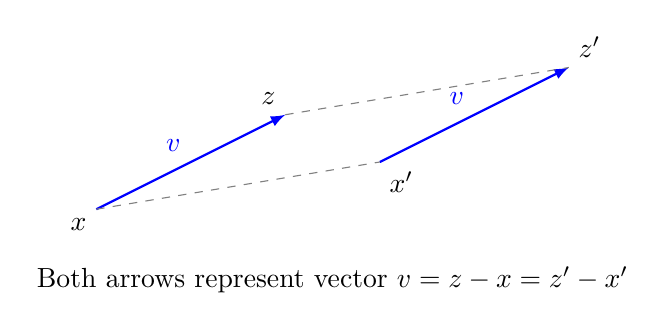
\begin{tikzpicture}[scale=1.2]
    % Define points
    \coordinate (x) at (0,0);
    \coordinate (z) at (2,1);
    \coordinate (xp) at (3,0.5);
    \coordinate (zp) at (5,1.5);
    
    % Draw arrows
    \draw[-latex, thick, blue] (x) -- (z) node[midway, above left] {$v$};
    \draw[-latex, thick, blue] (xp) -- (zp) node[midway, above left] {$v$};
    
    % Draw parallelogram
    \draw[dashed, gray] (x) -- (xp);
    \draw[dashed, gray] (z) -- (zp);
    
    % Label points
    \node[below left] at (x) {$x$};
    \node[above left] at (z) {$z$};
    \node[below right] at (xp) {$x'$};
    \node[above right] at (zp) {$z'$};
    
    % Show that both arrows represent the same vector
    \node[below] at (2.5, -0.5) {Both arrows represent vector $v = z - x = z' - x'$};
\end{tikzpicture}
\end{center}

\subsection{Equivalence Class Identification}
The relation $\sim$ partitions the space of all ``arrows'' into disjoint sets called \textbf{equivalence classes}. Each equivalence class corresponds to a unique vector $v \in \mathbb{R}^n$.
Specifically, the equivalence class of the pair $(0, v)$ contains all pairs $(x, z)$ such that $z-x = v-0 = v$.
Thus, we can identify the vector $v$ with the class of all arrows formed by such pairs.

\subsection{Worked Example: Equivalent Arrows in $\mathbb{R}^2$}
Consider the following pairs of points in $\mathbb{R}^2$:
\begin{itemize}
    \item $(x_1, z_1) = ((1, 2), (4, 5))$
    \item $(x_2, z_2) = ((0, 0), (3, 3))$
    \item $(x_3, z_3) = ((-1, 1), (2, 4))$
\end{itemize}

We compute the displacement vectors:
\begin{align*}
z_1 - x_1 &= (4, 5) - (1, 2) = (3, 3) \\
z_2 - x_2 &= (3, 3) - (0, 0) = (3, 3) \\
z_3 - x_3 &= (2, 4) - (-1, 1) = (3, 3)
\end{align*}

Since all three pairs yield the same displacement vector $(3, 3)$, they all belong to the same equivalence class. They represent the same vector $v = (3, 3)$, even though the arrows start and end at different locations.

\section{Geometric Properties}
A property $\mathcal{P}$ of subsets of $\mathbb{R}^n$ is called a \textbf{geometric property} (with respect to translations) if it is invariant under translation.
That is, if a set $K$ has property $\mathcal{P}$, then for any shift $y$, the set $K+y$ also has property $\mathcal{P}$.
\textbf{Examples:}
\begin{itemize}
    \item ``Being a sphere'' is a geometric property.
    \item ``Containing the origin'' is \textbf{not} a geometric property (since shifting it might move the origin outside).
\end{itemize}
This formalism allows us to distinguish between intrinsic properties of a shape (like volume, shape type) and extrinsic properties (like position).

\section{Chapter Summary}

In this chapter, we established the geometric foundations for working in $\mathbb{R}^n$:

\textbf{Key Definitions:}
\begin{itemize}
    \item \textbf{Translation/Shift:} The map $S_y(x) = x + y$ that shifts space by vector $y$
    \item \textbf{Congruence by Translation:} $K \cong_T L$ if $\exists y: K+y = L$
    \item \textbf{Vector as Equivalence Class:} Vectors are equivalence classes of arrows under the relation $(x,z) \sim (x',z') \iff z-x = z'-x'$
    \item \textbf{Geometric Property:} A property invariant under translations
\end{itemize}

\textbf{Key Results:}
\begin{itemize}
    \item The relation $\sim$ is an equivalence relation (reflexive, symmetric, transitive)
    \item Each equivalence class corresponds to a unique vector in $\mathbb{R}^n$
    \item Geometric properties capture the intrinsic nature of shapes, independent of position
\end{itemize}

These concepts provide the foundation for defining norms and distances in Chapter 2, which in turn enable the O notation (Chapter 3) and derivative definitions (Chapter 4).
